%!TEX root = IntroArithGrps.tex

\mychapter{Mostow Rigidity Theorem}
\label{MostowChap}

\prereqs{Quasi-isometries (\cref{QuasiChap}).}

%\begin{narrower} \hyphenpenalty=3000
%\em The Mostow Rigidity Theorem plays a fundamental role in nearly every paper on the geometry of Lie groups, and the techniques and ideas [Mostow] % he @@@
% introduced have influenced a lot of further work in geometry, group theory and dynamics.
%\\ \hbox{ } \hfil --- Yair Minsky, Yale University\break
%% \hbox{ } \hfil on the awarding of the Wolf Prize to G.\,D.\,Mostow in January 2013\break
%\par \end{narrower}


\section{Statement of the theorem}

In its simplest form, the Mostow Rigidity Theorem says that a single group~$\Gamma$ cannot be a lattice in two different semisimple groups~$G_1$ and~$G_2$ (except for  minor modifications involving compact factors, the center, and passing to a finite-index subgroup):

\begin{thm}[(Weak version of the Mostow Rigidity Theorem)] \label{MostowIso}
	\thmindex{Mostow Rigidity!weak version}
Assume
\noprelistbreak
	\begin{itemize}
	\item $G_1$ and~$G_2$ are connected, with trivial center and no compact factors,
	and
	\item $\Gamma_i$ is a lattice in~$G_i$, for $i = 1,2$.
	\end{itemize}
If\/ $\Gamma_1 \iso \Gamma_2$, then $G_1 \iso G_2$.
\end{thm}

In other words, if there is an isomorphism from~$\Gamma_1$ to~$\Gamma_2$, then there is also an isomorphism from~$G_1$ to~$G_2$. In fact, it is usually the case that something much stronger is true: 
%if no simple factor of~$G_1$ is isogenous to $\SL(2,\real)$, then every isomorphism between~$\Gamma_1$ and~$\Gamma_2$ actually comes from an isomorphism between $G_1$ and~$G_2$:

\begin{namedthm}[Mostow Rigidity Theorem]
\label{MostowRigidity}
Assume
\noprelistbreak
	\begin{itemize}
	\item $G_1$ and~$G_2$ are connected, with trivial center and no compact factors,
	\item $\Gamma_i$ is a lattice in~$G_i$, for $i = 1,2$,
	and
	\item there does not exist a simple factor~$N$ of~$G_1$, such that $N \iso \PSL(2,\real)$ and $N \cap \Gamma_1$ is a lattice in~$N$.
	\end{itemize}
Then any isomorphism from~$\Gamma_1$ to~$\Gamma_2$ extends
to a continuous isomorphism from~$G_1$ to~$G_2$.
 \end{namedthm}


\begin{rems}  \ \label{MostowRems}
\noprelistbreak
	\begin{enumerate}

	\item \label{MostowRems-deformationrigidity}
	Assume $G$ is connected, and has no simple factors that are either compact or isogenous to $\SL(2,\real)$. Then the Mostow Rigidity Theorem implies that lattices in~$G$ have no nontrivial deformations. More precisely, if $\Gamma_t$ is a continuous family of lattices in~$G$, then $\Gamma_t$ is conjugate to~$\Gamma_0$, for every~$t$ \csee{deformationrigidityEx}. 

This is not always true when $G$ is isogenous to $\SL(2,\real)$ \csee{ModuliSpaceSL2}, which explains why the statement of the Mostow Rigidity Theorem must forbid factors that are isogenous to $\SL(2,\real)$.

	\item In geometric terms, the Mostow Rigidity Theorem tells us that the topological structure of any irreducible finite-volume locally symmetric space of noncompact type completely determines its geometric structure as a Riemannian manifold (up to multiplying the metric by a scalar on each irreducible factor of the universal cover), if the manifold is not $2$-dimensional \ccf{MostowGeomEx}.


	\item \label{MostowRems-FurmanRigidity}
%\Cref{MostowIso} tells us that if we ignore some obvious minor modifications coming from compact groups, then $\Gamma$ does not embed as a lattice in any connected, semisimple Lie group other than~$G$. However, $\Gamma$~is also a lattice in a quite different Lie group; namely, $\Gamma$~is a lattice in itself.
%
	Assume $\Gamma$ is cocompact in~$G$. Then, as a strengthening of \cref{MostowIso}, it can be shown that if $\Gamma$ is a cocompact lattice in some Lie group~$H$ (not assumed to be semisimple), then $H$ must be either $G$ or~$\Gamma$ (modulo the usual minor modifications involving compact groups). In fact, this remains true even if we allow~$H$ to be any locally compact group, not necessarily a Lie group.

	\end{enumerate}
\end{rems}



\begin{exercises}

\item Suppose 
	\begin{itemize}
	\item $G$ has trivial center and no compact factors,
	\item  $G \not\iso \PSL(2,\real)$,
	and
	\item $\Gamma$ is irreducible. 
	\end{itemize}
Show that every automorphism of~$\Gamma$ extends to a continuous automorphism of~$G$.

\item Show that \cref{MostowIso} is a corollary of \cref{MostowRigidity}.
\hint{This is obvious when no simple factor of~$G_1$ is isomorphic to $\PSL(2,\real)$. The problem can be reduced to the case where $G_1$ and~$G_2$ are irreducible.}

\item \label{NotIsoForCpctFactors}
Assume $G_1$ and~$G_2$ are isogenous. Show that if $K$ is any compact group, then some lattice in~$G_1$ is isomorphic to a lattice in $G_2 \times K$ (even though $G_1$ may not be isomorphic to $G_2 \times K$). This is why \cref{MostowIso} assumes $G_1$ and~$G_2$ are connected, with trivial center and no compact factors
\hint{Any torsion-free lattice in~$G_1^\circ$ is isomorphic to a lattice in $G_2 \times K$.}

\item For $i = 1,2$, suppose 
	\begin{itemize}
	\item $\Gamma_i$ is a lattice in~$G_i$, 
	and 
	\item $G_i$ is connected and has no compact factors. 
	\end{itemize}
Show that if $\Gamma_1$ is isomorphic to~$\Gamma_2$, then $G_1$ is isogenous to~$G_2$.

\item Let $\Gamma_i$ be a lattice in~$G_i$ for $i = 1,2$. Show that if $\Gamma_1 \iso \Gamma_2$, then there is a compact, normal subgroup~$K_i$ of~$G_i^\circ$, for $i = 1,2$, such that $G_1^\circ/K_1 \iso G_2^\circ/K_2$.

%\item Let $G_1 = \SL(4,\real)$ and $G_2 = \PSL(4,\real)$. 
%\begin{enumerate}
%\item Show $G_1 \not\iso G_2$.
%\item Show there exist lattices $\Gamma_1$ and~$\Gamma_2$ in $G_1$ and~$G_2$, respectively, such that $\Gamma_1 \iso \Gamma_2$.
%\item Why is this not a counterexample to \cref{MostowRigidity}?
%\end{enumerate}

\item Let $G = \PSL(2,\real)$. 
Find an automorphism~$\varphi$ of some lattice~$\Gamma$ in~$G$, such that $\varphi$ does not extend to an automorphism of~$G$.
\par
Why is this not a counterexample to \cref{MostowRigidity}?

%\item Let $G_1 = \PSO(2,3)$ and $G_2 = \PSO(2,3) \times \PSO(5)$. 
%\begin{enumerate}
%\item Show $G_1 \not\iso G_2$.
%\item Show there exist irreducible lattices $\Gamma_1$ and~$\Gamma_2$ in $G_1$ and~$G_2$, respectively, such that $\Gamma_1 \iso \Gamma_2$.
%\item Why is this not a counterexample to \cref{MostowRigidity}?
%\end{enumerate}

%\item In the statement of \cref{MostowRigidity}:
%\begin{enumerate}
%\item Show the assumption that $\Gamma_1$ is irreducible can be replaced with the assumption that $\Gamma_2$ is irreducible.
%\item Show the assumption that $\Gamma_1$ is irreducible can be replaced with assumption that no simple factor of~$G_1$ is isomorphic to $\PSL(2,\real)$.
%\end{enumerate}

%\item \label{TrivialDeformEx}
%Verify that the construction of \cref{TrivialDeformLatt} defines a continuous deformation of~$\Gamma$.

\item \label{deformationrigidityEx}
Assume there is a continuous function $\rho \colon \Gamma \times [0,1] \to G$, such that, if we let $\rho_t(\gamma) = \rho(\gamma,t)$, then:
 	\begin{itemize}
	\item $\rho_t$ is a homomorphism, for all~$t$,
	\item $\rho_t(\Gamma)$ is a lattice in~$G$, for all~$t$,
	and
	\item $\rho_0(\gamma) = \gamma$, for all~$\gamma \in \Gamma$.
	\end{itemize}
Show that if $G$ is as in the first sentence of \fullcref{MostowRems}{deformationrigidity}, then $\Gamma_t$ is conjugate to~$\Gamma$, for every~$t$.
\hint{Reduce to the case where $G$ has trivial center. You may use, without proof, the fact that the identity component of the automorphism group of~$G$ consists of inner automorphisms \csee{OutGFinite}.}

\item \label{MostowGeomEx}
(\emph{Requires some familiarity with locally symmetric spaces})
Assume, for $i = 1,2$:
	\begin{itemize}
	\item $G_i$ is connected and simple, with trivial center,
	\item $K_i$ is a maximal compact subgroup of~$G_i$,
%	\item $X_i = K_i \backslash G_i$ is the symmetric space associated to~$G_i$,
	\item $\Gamma_i$ is a torsion-free, irreducible lattice in~$G_i$,
	\item $X_i = K_i \backslash G_i / \Gamma_i$ is the corresponding locally symmetric space of finite volume,
	\item the metric on~$X_i$ is normalized so that $\vol(X_1) = 1$,
	and
	\item $\dim X_1 \ge 3$.
	\end{itemize}
Show that any homotopy equivalence from~$X_1$ to~$X_2$ is homotopic to an isometry.
\hint{Since the universal cover $K_i \backslash G_i$ is contractible, a homotopy equivalence is determined, up to homotopy, by its effect on the fundamental group.}

\end{exercises}



\section{Sketch of the proof for \texorpdfstring{$\SO(1,\lowercase{n})$}{SO(1,n)} 
\texorpdfstring{\optional}{(optional)}} \label{MostowPfSect}

In most cases, the conclusion of the Mostow Rigidity Theorem \pref{MostowRigidity} is an easy consequence of the \thmindex{Margulis!Superrigidity}{Margulis Superrigidity Theorem}, which will be discussed in \cref{MargulisSuperChap}.
More precisely, if we assume, for simplicity, that the lattices $\Gamma_1$ and~$\Gamma_2$ are irreducible \csee{MostowRigIrredEnough}, then the Margulis Superrigidity Theorem applies unless $G_1$ and~$G_2$ are isogenous to either $\SO(1,n)$ or $\SU(1,n)$ \csee{ProveMostMostowEx}.
To illustrate the main ideas involved in completing the proof, we discuss a special case:

\begin{proof}[\mathversion{bold}Proof  of Mostow Rigidity Theorem for cocompact lattices in $\SO(1,n)$]
Assume, for $i = 1,2$:
\noprelistbreak
	\begin{itemize}
	\item $G_i \iso \PSO(1,n_i)$, for some $n_i \ge 3$,
	\item $\Gamma_i$ is cocompact in~$G_i$,
	and
	\item $\rho \colon \Gamma_1 \to \Gamma_2$ is an isomorphism.
	\end{itemize}
In order to show that $\rho$ extends to a continuous homomorphism from $G_1$ to~$G_2$, we take a geometric approach that uses the action of $G_i$ on its associated symmetric space, which is the hyperbolic space~$\hyperbolic^{n_i}$.
This assumes some understanding of hyperbolic space (and other matters) that is not required elsewhere in this book.

\begin{claim}
We have $n_1 = n_2$.
\end{claim}
By passing to subgroups of finite index, we may assume $\Gamma_1$ and~$\Gamma_2$ are torsion free, so $\Gamma_i$ acts freely on~$\hyperbolic^{n_i}$. The action is also properly discontinuous, so, since hyperbolic space is contractible, this implies that $X_i = \Gamma_i \backslash \hyperbolic^{n_i}$ is a $K(\Gamma_i, 1)$-space. Since $X_i$ is a compact manifold of dimension~$n_i$, we conclude that the cohomological dimension of~$\Gamma_i$ is~$n_i$. However, the groups $\Gamma_1$ and~$\Gamma_2$ are isomorphic, so they must have the same cohomological dimension. This completes the proof of the claim.
\qed

\medbreak

Therefore, $\Gamma_1$ and~$\Gamma_2$ are two lattices in the same group $G = \PSO(1,n)$. To simplify matters, let us assume $n = 3$.

Since $\Gamma_i$ is cocompact in~$G_i$ (so $\Gamma_i$ is quasi-isometric to~$\hyperbolic^3$), it is not difficult to construct a quasi-isometry $\varphi \colon \hyperbolic^3 \to \hyperbolic^3$, such that
	\begin{align} \label{MostowPfSO13Equi}
	\text{$\varphi(\gamma x) = \rho(\gamma) \cdot \varphi(x)$ 
	\ for all $\gamma \in \Gamma_1$ and $x \in \hyperbolic^3$} 
	\end{align}
\csee{MostowPfSO13EquiEx}.

Consider the ball model of~$\hyperbolic^3$, whose boundary $\bdry \hyperbolic^3$ is the round $2$-sphere~$S^2$. It is easy to see that any isometry~$\phi$ of~$\hyperbolic^3$ induces a well-defined homeomorphism $\overline\phi$ of $\bdry \hyperbolic^3$. 
Furthermore, it is well known that this boundary map is \defit{conformal} (i.e., it is angle-preserving). This implies that if $C$ is a very small circle in $\bdry \hyperbolic^3$, then $\overline\phi(C)$ is very close to being a circle; more precisely, if we let $S_r(p)$ be the sphere of radius~$r$ around the point~$p$, then
	$$ \limsup_{r \to 0^+} \frac{\sup_{x \in S_r(p)} d \bigl( \overline\phi(x), \overline\phi(p) \bigr)}{\inf_{y \in S_r(p)} d \bigl( \overline\phi(y), \overline\phi(p) \bigr)}
	= 1 .$$
With this background in mind, it should not be difficult to believe (and it is not terribly difficult to prove) that the quasi-isometry $\varphi$ induces a well-defined homeomorphism $\overline\varphi$ of $\bdry \hyperbolic^3$, such that 
	\begin{align} \label{MostowPfSO13OverlineVarphi}
	\text{$\overline\varphi(\gamma p) = \overline{\rho(\gamma)} \cdot \overline\varphi(p)$ 
	\ for all $\gamma \in \Gamma_1$ and $p \in \bdry\hyperbolic^3$} 
	. \end{align}
Furthermore, this boundary map is \defit[quasi-!conformal]{quasi-conformal}, which means that if $C$ is a very small circle in $\bdry \hyperbolic^3$, then $\overline\varphi(C)$ is approximated by an ellipse of bounded eccentricity; more precisely, there is some constant $\kappa > 0$, such that, for all $p \in \bdry \hyperbolic^3$, we have
	$$ \limsup_{r \to 0^+} \frac{\sup_{x \in S_r(p)} d \bigl( \overline\varphi(x), \overline\varphi(p) \bigr)}{\inf_{y \in S_r(p)} d \bigl( \overline\varphi(y), \overline\varphi(p) \bigr)}
	< \kappa .$$ 

It is a fundamental, but highly nontrivial, fact that quasi-conformal maps are differentiable almost everywhere. Therefore, if $C_p$ is a circle (centered at the origin) in the tangent plane at almost any point $p \in \bdry\hyperbolic^3$, then $\overline\varphi(C_p)$ is an ellipse in the tangent plane at $\overline\varphi(p)$. Furthermore, since multiplying all the vectors in a tangent plane by a scalar does not change the eccentricity of any ellipse in the plane, we see that the eccentricity $e_p$ of this ellipse is independent of the choice of the circle~$C_p$. So~$e_p$ is a well-defined, measurable function on (almost all of)~$\bdry\hyperbolic^3$.

\setcounter{case}{0}

\begin{case}
Assume $e_p = 1$ for almost all $p \in \bdry\hyperbolic^3$.
\end{case}
This implies that the quasi-conformal map~$\overline\varphi$ is actually conformal. So there is an isometry~$\alpha$ of~$\hyperbolic^3$, such that $\overline\alpha = \overline\phi$. Then, for $\gamma \in \Gamma_1$ and $p \in \bdry\hyperbolic^3$, we have
	$$ \overline\alpha( \gamma p)
	= \overline\varphi( \gamma p)
	= \overline{\rho(\gamma)} \cdot \overline\varphi(p)
	= \overline{\rho(\gamma)} \cdot \overline\alpha(p)
	. $$
On the other hand, since $G$ is the identity component of $\Isom(\hyperbolic^3)$, it is normalized by~$\alpha$, so there is an automorphism $\widehat\alpha$ of~$G$, such that, for all $g \in G$ and $p \in \bdry\hyperbolic^3$, we have
	$$ \overline\alpha(gp) = \overline{\widehat\alpha(g)} \cdot \overline\alpha(p) .$$
By comparing the displayed equations (and letting $g = \gamma$), we see that $\widehat\alpha(\gamma) = \rho(\gamma)$ for all $\gamma \in \Gamma_1$. Therefore, $\widehat\alpha$ is the desired extension of~$\rho$ to an isomorphism defined on all of~$G$.

\begin{case} \label{MostowPfSO13Not1}
Assume $e_p$ is not almost always equal to~$1$.
\end{case}
Since $\overline{\rho(\gamma)}$ is conformal (because $\rho(\gamma)$ is an isometry), we see from \pref{MostowPfSO13OverlineVarphi} that $e_{\gamma p} = e_p$ for all $\gamma \in \Gamma_1$ and (almost) all $p \in \bdry\hyperbolic^3$. However, since $\overline{G}$ is transitive on $\bdry\hyperbolic^3$ with noncompact point-stabilizers, the Moore Ergodicity Theorem \pref{GammaErgOnG/H} implies that $\overline{\Gamma_1}$ is ergodic on $\bdry\hyperbolic^3$, so we conclude that the function $e_p$ is  constant (a.e). 

Thus, the assumption of this \lcnamecref{MostowPfSO13Not1} implies that, for almost every~$p$, the ellipse $\overline\varphi(C_p)$ is not a circle, and therefore has a well-defined major axis~$\ell_p$, which is a line through the origin in the tangent plane at~$\overline\varphi(p)$. Hence, $\{\ell_p\}$ is a (measurable) section of a certain bundle $\mathbf{P}\hyperbolic^3$, namely, the $\real \mathbf{P}^1$-bundle over $\hyperbolic^3$ whose fiber at each point is the projectivization of the tangent space. Furthermore, since $\overline{\Gamma_2} = \overline{\rho(\Gamma_1)}$ is conformal, we see from \pref{MostowPfSO13OverlineVarphi} that this section is $\overline{\Gamma_2}$-invariant. In fact, if we rotate $\{\ell_p\}$ by any angle~$\theta$, then the resulting section $\{\ell_p^\theta\}$  is also invariant (since $\overline{\Gamma_2}$ is conformal). Then $\bigcup_{0 \le \theta \le \pi/2} \{\ell_p^\theta\}$ is a measurable, $\overline{\Gamma_2}$-invariant subset of $\mathbf{P}\hyperbolic^3$. However, the Moore Ergodicity Theorem \pref{GammaErgOnG/H} implies there are no such (nontrivial) subsets, since $\overline{G}$ is transitive on $\mathbf{P}\hyperbolic^3$ with noncompact point-stabilizers. This contradiction completes the proof, by showing that this \lcnamecref{MostowPfSO13Not1} does not occur.
\end{proof}

\begin{rems} \label{MostowPfRems} \ 
\noprelistbreak
	\begin{enumerate}
	\item The above proof makes the simplifying assumption that $n = 3$. Essentially the same proof works for larger values of~$n$, but $\overline\varphi(C_p)$ will be an ellipsoid, rather than an ellipse, so the space $\ell_p$ of major directions may be a higher-dimensional subspace of the tangent space, instead of just being a line.

	\item \label{MostowPfRems-QuasiC}
	Mostow was able to modify the proof to deal with $\SU(1,n)$, instead of $\SO(1,n)$, by developing a theory of  maps that are quasiconformal over~$\complex$. (In fact, replacing $\complex$ with the quaternions and octonions yields proofs for lattices in  the other simple groups of real rank one, namely, $\Sp(1,n)$ and $F_{4,1}$. However, this is not necessary, because the Margulis Superrigidity Theorem applies to these groups.)

	\item \label{MostowPfRems-Qrank1}
	For lattices in $\SO(1,n)$ that are \textbf{not} cocompact, it is not at all obvious that an isomorphism $\Gamma_1 \iso \Gamma_2$ should yield a quasi-isometry $\hyperbolic^n \to \hyperbolic^n$. This was proved by G.\,Prasad, by using the ``\term{Siegel set}'' description of a coarse fundamental domain for the action of~$\Gamma_i$ on $\hyperbolic^n$ \ccf{ReductionChap}. 
	The same method also works for noncocompact lattices in $\SU(1,n)$, or, more generally, whenever $\Qrank \Gamma_1 = 1$.
	\end{enumerate}
\end{rems}

\begin{exercises}

\item \label{MostowRigIrredEnough}
Show that the proof of \cref{MostowRigidity} can be reduced to the special case where the lattices $\Gamma_1$ and~$\Gamma_2$ are irreducible in $G_1$ and~$G_2$, respectively.
In other words, assume the conclusion of \cref{MostowRigidity} holds whenever $\Gamma_i$ is irreducible in~$G_i$, for $i = 1,2$, and show that this additional hypothesis can be eliminated.

\item \label{MostowPfSO13EquiEx}
Construct a quasi-isometry $\varphi \colon \hyperbolic^3 \to \hyperbolic^3$ that satisfies \pref{MostowPfSO13Equi}.
\hint{Let $\fund$ be a precompact strict fundamental domain for the action of~$\Gamma_1$ on~$\hyperbolic^3$, and choose some $x_0 \in \hyperbolic^3$. For $x \in \hyperbolic^3$, let $\varphi(x) = \rho(\gamma)x_0$, where $x \in \gamma \cdot \fund$.}

\end{exercises}











\section{Moduli space of lattices in \texorpdfstring{$\SL(2,\real)$}{SL(2,R)}} \label{ModuliSpaceSL2}

Suppose $\Gamma$ is a torsion-free, cocompact lattice in $\SL(2,\real)$. In contrast to the Mostow Rigidity Theorem \pref{MostowRigidity}, we will see that an isomorphism $\Gamma \iso \Gamma'$ need not extend to an automorphism of $\SL(2,\real)$. In fact, there are uncountably many different embeddings of~$\Gamma$ in $\SL(2,\real)$ that are not conjugate to each other.

To see this, we take a geometric approach.
Since $\SL(2,\real)$ acts transitively on the hyperbolic plane~$\hyperbolic^2$ (by isometries), the quotient $\Gamma \backslash \hyperbolic^2$ is a compact surface~$M$. We will show there are uncountably many different possibilities for~$M$ (up to isometry). 
The proof is based on the fact that the hyperbolic plane has uncountably many different right-angled hexagons.

\begin{lem} \label{ManyHexagons}
The hyperbolic plane\/~$\hyperbolic^2$ has uncountably many different right-angled hexagons \textup(no two congruent to each other\/\textup).
\end{lem}

\begin{proof}
Fix a basepoint $p \in \hyperbolic^2$, and a starting direction~$\vector v$. For $\vector s \in (\real^+)^6$, construct the piecewise-linear path $L = L(\vector s)$ in~$\hyperbolic^2$ determined by:

\begin{minipage}{2.2in} %{% no page break in this paragraph !!!
	\raggedright
	\vbox to -3pt{\vskip 0.075in \rightline{\hbox to 0pt{\hskip8pt 
		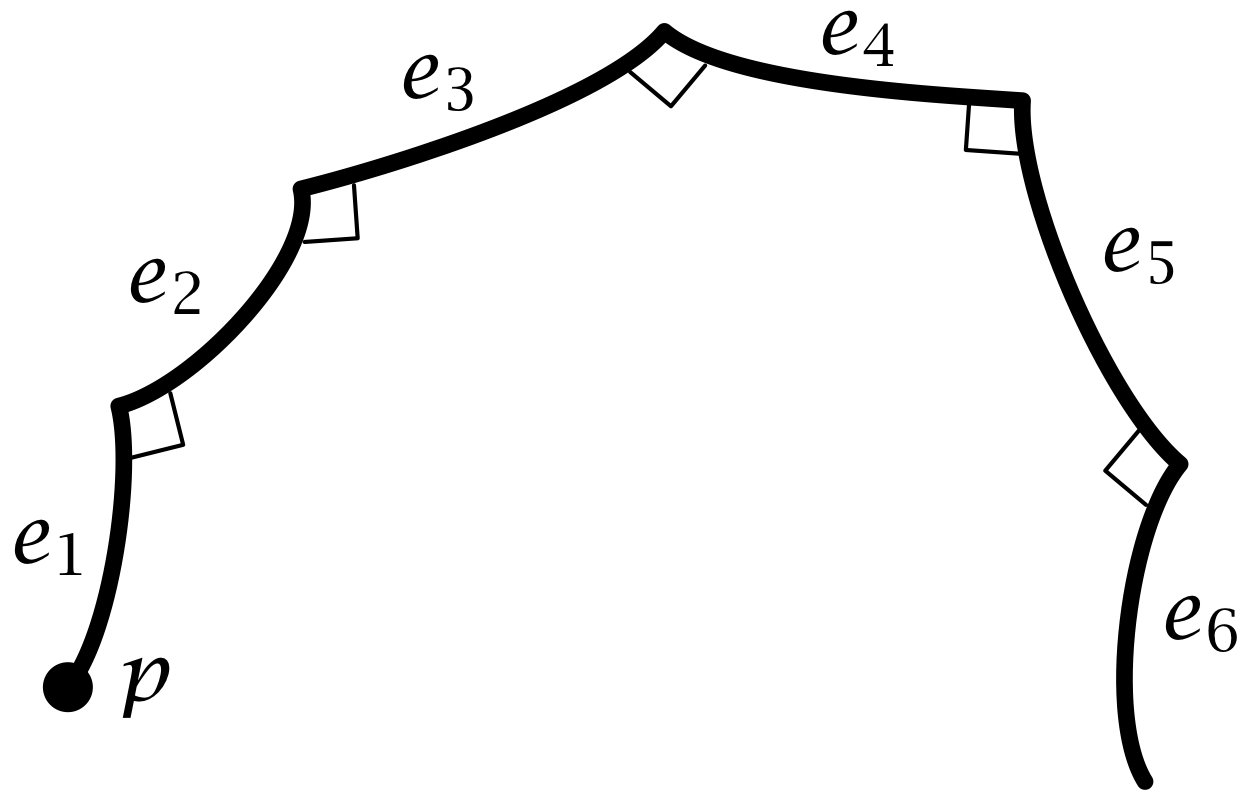
\includegraphics{PDF/path6.jpg}\hss}}\vss}
%texpreamble
%("  \usepackage{amsmath}
% \usepackage[LY1]{fontenc}
% \usepackage[expert,LY1,mylucidascale]{mylucidabr}
% ");
%defaultpen(  fontcommand("\normalfont") + fontsize(10) ); 
%
%from graph access *;
%unitsize(1.5cm);
%
%real linethick = 1.5;
%real dotthick = 12;
%dotfactor=12;
%
%real pi = 3.14159265;
%pair[] p = {(0,0), (-0.4,0.7), (-0.4,1.5), (0.1,2.5), (1,3), (2,2.5), (2.5,1.75) } ;
%pair[] v;
%real[] t= {pi/2 ,0.8*pi, 0.8*pi, 0.5*pi, 0.2*pi, 0, -0.1*pi};
%
%v[0] = (0,1);
%for (int i = 1 ; i <=6; ++i)
%	{v[i] = (cos(t[i]), sin(t[i]) );}
%
%
%// picture goes to high -- rotate everything by 40 degrees
%for (int i = 0; i <= 6; ++i){\
%	p[i] = rotate(-40)*p[i] ;
%	v[i] = rotate(-40)*v[i] ;
%	t[i] = t[i] - pi*40/180;
%	}
%
%draw( p[0]
%	{v[0]}..tension(1.5)..{v[1]}
%	p[1]
%	{rotate(-90)*v[1]}..tension(1.5)..{v[2]}
%	p[2]
%	{rotate(-90)*v[2]}..tension(1.5)..{v[3]}
%	p[3]
%	{rotate(-90)*v[3]}..tension(1.5)..{v[4]}
%	p[4]
%	{rotate(-90)*v[4]}..tension(1.5)..{v[5]}
%	p[5]
%	{rotate(-90)*v[5]}..tension(1.5)..{v[6]}
%	p[6],
%	linewidth(2)
%	);
%
%label( "$e_1$",0.5*(p[0] + p[1]) , 0.01*W );
%label( "$e_2$", 0.5*(p[1] + p[2]) , 0.01*WNW );
%label( "$e_3$", 0.5*(p[2] + p[3]) , 0.01*NW );
%label( "$e_4$", 0.5*(p[3] + p[4]) , 0.01*NNE );
%label( "$e_5$", 0.5*(p[4] + p[5]) , 0.01*NE );
%label( "$e_6$", 0.5*(p[5] + p[6]) , 0.01*E );
%
%draw( p[0], linewidth(6) );
%label( "$p$", p[0], 2*E );
%
%real r = 0.15;
%draw( shift(p[1])*(rotate(180 + (180*t[1]/pi))*( (r,0)--(r,r)--(0,r) ) ) );
%draw( shift(p[2])*(rotate(-10 + 180 + (180*t[2]/pi))*( (r,0)--(r,r)--(0,r) ) ) );
%draw( shift(p[3])*(rotate(180 + (180*t[3]/pi))*( (r,0)--(r,r)--(0,r) ) ) );
%draw( shift(p[4])*(rotate(180 + (180*t[4]/pi))*( (r,0)--(r,r)--(0,r) ) ) );
%draw( shift(p[5])*(rotate(180 + (180*t[5]/pi))*( (r,0)--(r,r)--(0,r) ) ) );
	\begin{itemize}
	\hangindent=-2.2in
	\hangafter=0
	\item The path starts at the point~$p$.
	\item \hangindent=-2in \hangafter=0
	 The path consists of $6$ geodesic segments (or ``edges'') $e_1,\ldots,e_6$, of lengths $s_1,\ldots,s_6$, respectively.\par
	\item The first edge~$e_1$ starts at~$p$ and heads in the direction~$\vector v$.
	\item For $i \ge 2$, edge~$e_i$ %is of length~$s_i$, and 
	makes a (clockwise) right angle with~$e_{i-1}$.
	\end{itemize}
\end{minipage}
\par\smallskip\noindent 
The variables $s_1,\ldots,s_6$ provide $6$~degrees of freedom in the construction of~$L$. Requiring that $L$ be a closed path (i.e., that the terminal endpoint of~$L$ is equal to~$p$) takes away two degrees of freedom (because $\hyperbolic^2$ is $2$-dimensional). Then, requiring the angle between $e_6$ and~$e_1$ to be right angle takes away one more degree of freedom. Hence (from the 
\thmindex{Implicit Function}{Implicit Function Theorem}), % should this be in the Background appendix? @@@
we see that there are $3$~degrees of freedom in the construction of a right-angled hexagon in~$\hyperbolic^2$. 
\end{proof}

\begin{rem} \label{AltEdgesInRtHex}
In fact, calculations using the trigonometry of triangles in~$\hyperbolic^2$ yields the much more precise fact that, for any $s_2,s_4,s_6 \in \real^+$, there exists a unique right-angled hexagon, with edges $e_1,\ldots,e_6$, such that the length of edge $e_{2i}$ is exactly~$s_{2i}$, for $i = 1,2,3$. (That is, the lengths of the three edges $e_2$, $e_4$, and~$e_6$ can be chosen completely arbitrarily, and they uniquely determine the lengths of the other three edges in the right-angled hexagon.)
\end{rem}

\begin{defn}
A \defit[hyperbolic!surface]{hyperbolic surface} is a compact Riemannian manifold (without boundary) whose universal cover is the hyperbolic plane~$\hyperbolic^2$.
\end{defn}

\begin{cor} \label{ManyHypSurfs}
There are uncountably many non-isometric hyperbolic surfaces of any given genus $g \ge 2$.
\end{cor}

\begin{proof}
Choose a right-angled hexagon~$P$ in~$\hyperbolic^2$. Call its edges $e_1,\ldots,e_6$, and let $s_i$ be the length of~$e_i$. Make a copy~$P'$ of~$P$, and form a surface~$\mathcal{P}$ by gluing $e_{2i}$ to the corresponding edge~$e_{2i}'$ of~$P'$, for $i = 1,2,3$. 
(Topologically, this surface~ $\mathcal{P}$ is a disk with two holes, and is usually called a ``pair of pants\zz.'')
$$ 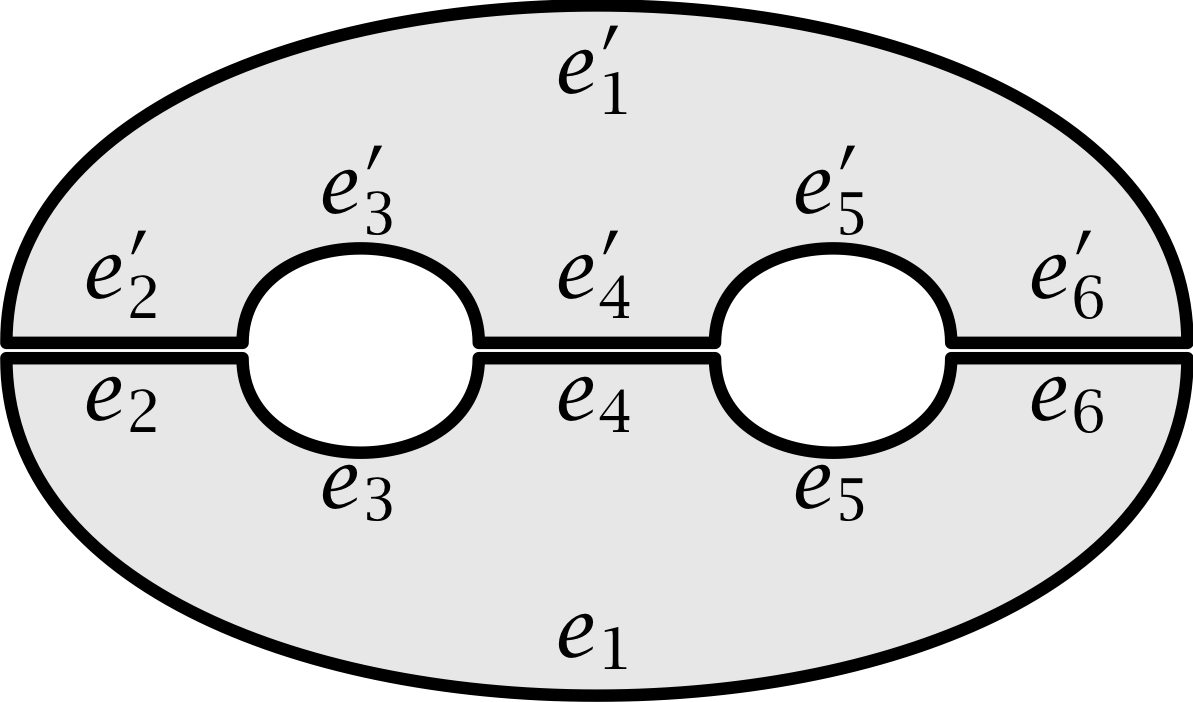
\includegraphics{PDF/twohexagons.jpg}
%texpreamble
%("  \usepackage{amsmath}
% \usepackage[LY1]{fontenc}
% \usepackage[expert,LY1,mylucidascale]{mylucidabr}
% ");
%defaultpen(  fontcommand("\normalfont") + fontsize(10) ); 
%
%from graph access *;
%unitsize(1cm);
%
%real linethick = 1.5;
%real dotthick = 12;
%dotfactor=12;
%
%
%// draw( rotate(60)*ellipse( (0,0), 1,2 ) ) ;
%
%real eps = -0.0325;
%
%filldraw(
%	(
%	(0,0)
%	{N}..tension(1.75)..{S}
%	(5,0)--(4,0)
%	{N}..tension(1.25)..{S}
%	(3,0)--(2,0)
%	{N}..tension(1.25)..{S}
%	(1,0)--cycle
%	),
%	gray(0.925),
%	linewidth(1.5)
%	);
%
%filldraw(
%	reflect((0,eps), (1,eps))*(
%	(0,0)
%	{N}..tension(1.75)..{S}
%	(5,0)--(4,0)
%	{N}..tension(1.25)..{S}
%	(3,0)--(2,0)
%	{N}..tension(1.25)..{S}
%	(1,0)--cycle
%	),
%	gray(0.925),
%	linewidth(1.5)
%	);
%
%label( "$e_6'$", (4.5,0), N );
%label( "$e_5'$", (3.5,0.65) );
%label( "$e_4'$", (2.5,0), N );
%label( "$e_3'$", (1.5,0.65) );
%label( "$e_2'$", (0.5,0), N );
%label( "$e_1'$", (2.5,1.45), S);
%
%label( "$e_6$", (4.5,-0 + eps), S );
%label( "$e_5$", (3.5,-0.6 + eps) );
%label( "$e_4$", (2.5,-0 + eps), S );
%label( "$e_3$", (1.5,-0.6 + eps) );
%label( "$e_2$", (0.5,-0 + eps), S );
%label( "$e_1$", (2.5,-1.45 + eps) , N );
\qquad
 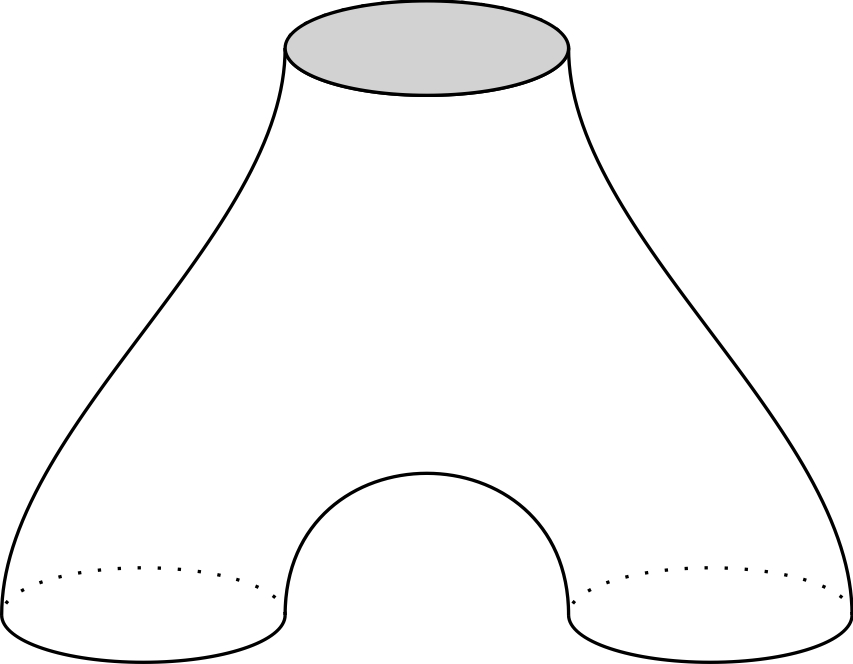
\includegraphics{PDF/pairofpants-fromwikipedia.jpg} $$
 % http://commons.wikimedia.org/wiki/File:Pair_of_pants_cobordism_%28pantslike%29.svg
 % @@@ I do not have asymptote code for this figure, since it was converted from svg to PDF
Since $P$ is right-angled, the three boundary curves of~$\mathcal{P}$ are geodesics. Their lengths are $2s_1$, $2s_3$, and~$2s_5$. 

\vbox{ % can't allow a page break in this paragraph !!!
\vbox to 0pt{\vskip 0.3in \rightline{$\begin{matrix}
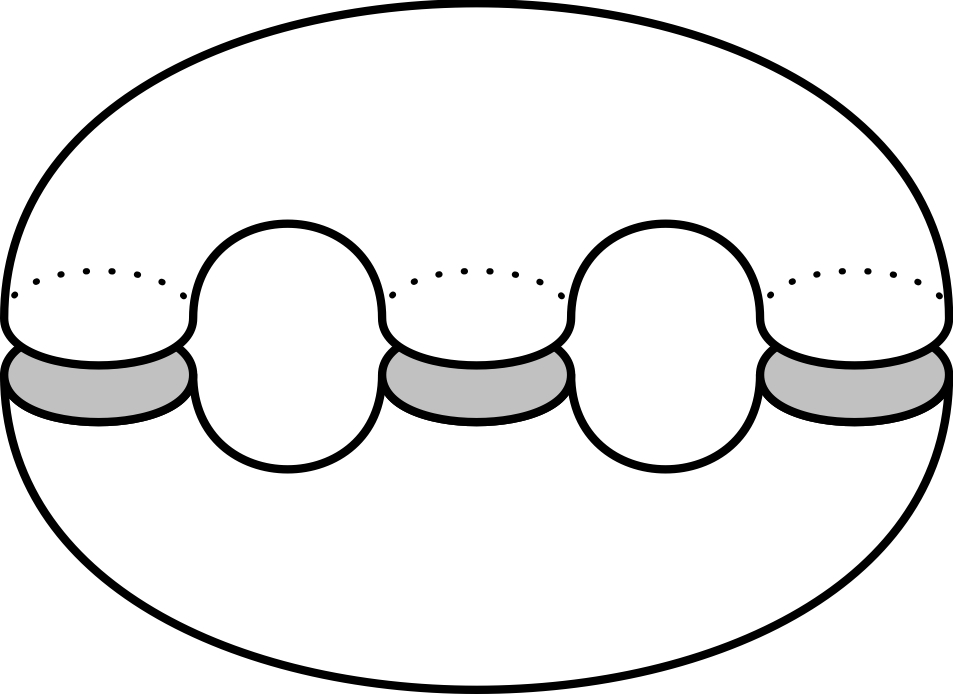
\includegraphics{PDF/genus2pants.jpg}
\\
\text{A surface of genus 2 can be} 
\\ \text{made from two pairs of pants.}
\end{matrix}
$}\vss}
%from graph access *;
%
%unitsize(0.4cm);
%
%currentpen=linewidth(1);
%
%real a = 0, b = 2, c = 4, d = 6, e = 8, f = 10;
%real z = -0.6;
%real s = 1;
%real t = 2;
%real gl = 0.8;
%real lw = 0.75;
%string lt = "3 3";
%
%
%draw(  (a,z){S}.. tension t .. {N}(b,z){S}..tension s ..{N}(c,z){S}..tension t ..{N}(d,z){S}..tension s ..{N}(e,z){S}..tension t ..{N}(f,z){S}.. tension 1.5 ..{N}cycle );
%
%
%
%filldraw( (a,z){S}.. tension t .. {N}(b,z){N}.. tension t .. {S}cycle , gray(gl) );
%filldraw( (c,z){S}.. tension t .. {N}(d,z){N}.. tension t .. {S}cycle , gray(gl) );
%filldraw( (e,z){S}.. tension t .. {N}(f,z){N}.. tension t .. {S}cycle , gray(gl) );
%
%
%filldraw(  (a,0){S}..tension t ..{N}(b,0){N}..tension s ..{S}(c,0){S}..tension t ..{N}(d,0){N}..tension s ..{S}(e,0){S}..tension t ..{N}(f,0){N}.. tension 1.5 ..{S}cycle, white );
%
%draw( (a,0){N}.. tension t ..{S}(b,0), linewidth(lw)+dotted );
%draw( (c,0){N}.. tension t ..{S}(d,0), linewidth(lw)+dotted );
%draw( (e,0){N}.. tension t ..{S}(f,0), linewidth(lw)+dotted );

\hangindent=-2.2in
\hangafter=0
Construct a closed surface~$M$ of genus~$2$ from two copies of~$\mathcal{P}$, by gluing corresponding boundary components to each other. 
(For a discussion of higher genus, see \cref{HigherGenusPants}.) Since the only curves that have been glued together are geodesics, it is easy to see that each point in~$M$ has a neighborhood that is isometric to an open subset of~$\hyperbolic^2$. Therefore, the universal cover of~$M$ is~$\hyperbolic^2$ (since $M$ is complete). So $M$ is a hyperbolic surface.
\par}

Furthermore, from the construction, we see that $M$ has a closed geodesic of length~$2s_1$. (In fact, there is a geodesic of length~$2s_i$, for $1 \le i \le 6$.) Since a single closed surface has closed geodesics of only countably many different lengths, but \cref{ManyHexagons} implies that there are uncountably many possible values of~$s_1$, this implies there must be uncountably many different isometry classes of surfaces.
\end{proof}

\begin{rem} \label{HigherGenusPants}
A hyperbolic surface~$M$ of any genus $g \ge 2$ can be constructed by gluing together $2g - 2$ pairs of pants:
$$ 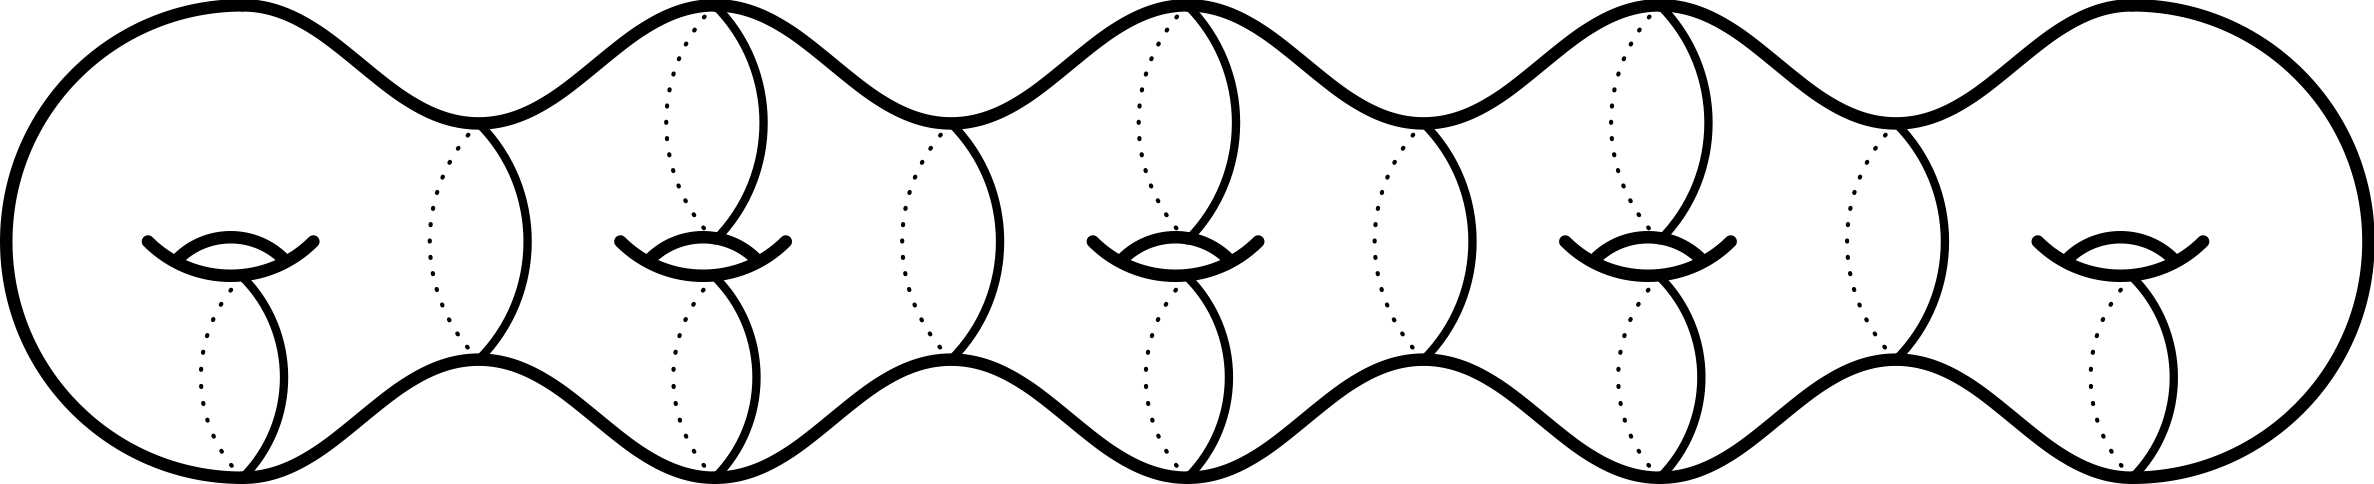
\includegraphics{PDF/highergenuspants.jpg} $$
The lengths of the three boundary curves of each pair of pants can be varied independently \ccf{AltEdgesInRtHex}, except that curves that will be glued together need to have the same length. The surface can also be modified by rotating any boundary curve through an arbitrary angle~$\theta$ before it is glued to its mate. This yields $6g-6$ degrees of freedom in the construction of~$M$. It can be shown that this is precisely the dimension of the space of hyperbolic surfaces of genus~$g$. In other words, $6g-6$ is the dimension of the \defit{moduli space} of hyperbolic surfaces of genus~$g$. 
\end{rem}
%texpreamble
%(" \usepackage[LY1]{fontenc}
% \usepackage[expert, LY1, mylucidascale]{mylucidabr} % I adjusted the scaling
% \usepackage{amsmath}
% \everymath{\displaystyle}
% ");
%defaultpen(  fontcommand("\normalfont") + fontsize(10) ); 
%
%from graph access *;
%
%unitsize(1cm);
%
%
%real a = 1, b = 0.5;
%
%currentpen=linewidth(1.5);
%draw( (1,-a){W}..(0,0)..{E}(1,a) );
%draw( (9,-a){E}..(10,0)..{W}(9,a) );
%for (int i = 1; i <= 7; i = i + 2){
%	draw( (i,a){E}..(i+1,b)..{E}(i+2,a) );
%	draw( (i,-a){E}..(i+1,-b)..{E}(i+2,-a) );
%	}
%
%for (int i = 0; i <= 8; i = i + 2 ){
%	currentpen=linewidth(1.5);
%	draw( (i + 0.6,0){SE}..{NE}(i + 1.3,0) );
%	draw( (i + 0.725,-0.075){NE}..{SE}(i + 1.175,-0.075) );
%
%	currentpen=linewidth(1);
%	draw( (i + 1, -0.15){(1,-1)}..{(-1,-1)}(i + 1,-a) );
%	draw( (i + 1, -0.15){(-1,-1)}..{(1,-1)}(i + 1,-a), dotted );
%	}
%
%currentpen=linewidth(1);
%
%for (int i = 3; i <= 7; i = i + 2 ){
%	draw( (i, 0.005){(1,1)}..{(-1,1)}(i,a) );
%	draw( (i, 0.005){(-1,1)}..{(1,1)}(i,a), dotted );
%	}
%
%for (int i = 2; i <= 8; i = i + 2 ){
%	draw( (i, -b){(1,1)}..{(-1,1)}(i,b) );
%	draw( (i, -b){(-1,1)}..{(1,1)}(i,b), dotted );
%	}

\begin{cor} \label{LotsOfLattsSL2}
If\/ $\Gamma$ is any lattice in\/ $\SL(2,\real)$, then there are uncountably many nonconjugate embeddings of\/~$\Gamma$ as a lattice in\/ $\SL(2,\real)$.
\end{cor}

\begin{proof}
Let us assume $\SL(2,\real)/\Gamma$ is compact. (Otherwise, $\Gamma$ is a free group, so it is easy to find embeddings.) Let us also assume, for simplicity, that $\Gamma$~is torsion free, so it is the fundamental group of the hyperbolic surface $\Gamma \backslash \hyperbolic^2$, which has some genus~$g$. Then $\Gamma$ is isomorphic to the fundamental group~$\Gamma'$ of any hyperbolic surface $\Gamma' \backslash \hyperbolic^2$ of genus~$g$. However, if $\Gamma \backslash \hyperbolic^2$ is not isometric to $\Gamma' \backslash \hyperbolic^2$, then $\Gamma$ cannot be conjugate to~$\Gamma'$ in the isometry group of~$\hyperbolic^2$. Therefore, \cref{ManyHypSurfs} implies that there must be uncountably many different conjugacy classes of subgroups~$\Gamma'$ that are isomorphic to~$\Gamma$.
\end{proof}




\section{Quasi-isometric rigidity} \label{QIRigSect}

The Mostow Rigidity Theorem's weak form \pref{MostowIso} tells us (under mild hypotheses) that lattices in two different semisimple Lie groups cannot be isomorphic. In fact, they cannot even be quasi-isometric \csee{QuasiIsomDefn}:

\begin{thm} \label{QI->GIso}
Assume
\noprelistbreak
	\begin{itemize}
	\item $G_1$ and~$G_2$ are connected, with trivial center and no compact factors,
	and
	\item $\Gamma_i$ is an irreducible lattice in~$G_i$, for $i = 1,2$.
	\end{itemize}
If\/ $\Gamma_1 \QI \Gamma_2$, then $G_1 \iso G_2$.
\end{thm}

Although nothing more than \cref{QI->GIso} can be said about quasi-isometric lattices that are cocompact \csee{CpctLattQI}, there is a much stronger conclusion for noncocompact lattices. Namely, not only are the Lie groups $G_1$ and~$G_2$ isomorphic, but the isomorphism can be chosen to make the lattices commensurable (unless $G_1 = G_2 = \PSL(2,\real)$): 

\begin{thm} \label{QuasiMostowRig}
Assume
\noprelistbreak
	\begin{itemize}
	\item $G_1$ and~$G_2$ are connected, with trivial center and no compact factors,
	and
	\item $\Gamma_i$ is an irreducible lattice in~$G_i$, for $i = 1,2$.
	\end{itemize}
Then\/ $\Gamma_1 \QI \Gamma_2$ if and only if
$G_1 \iso G_2$ and either
 \begin{enumerate}
 \item both $G_1/\Gamma_1$ and $G_2/\Gamma_2$ are compact, or
 \item there is an isomorphism $\phi \colon G_1 \to G_2$,
such that $\phi(\Gamma_1)$ is commensurable
to\/~$\Gamma_2$, or
 \item $G_1$ and $G_2$ are isomorphic to\/ $\PSL(2,\real)$,
and neither $G_1/\Gamma_1$ nor $ G_2/\Gamma_2$ is compact.
 \end{enumerate}
 \end{thm}
 
%We will say a little about its proof later in the section. 
One of the key ingredients in the proof of this \lcnamecref{QuasiMostowRig} is the fact that any group quasi-isometric to a lattice is isomorphic to a lattice, modulo finite groups:

\begin{thm} \label{QItoLatt}
 If $\Lambda$ is a finitely generated group that is quasi-isometric to an irreducible lattice\/~$\Gamma$ in~$G$, then there are
 	\begin{itemize}
	\item a finite-index subgroup~$\Lambda'$ of~$\Lambda$,
	and
	\item a finite, normal subgroup~$N$ of~$\Lambda'$, 
	\end{itemize}
such that $\Lambda'/N$ is isomorphic to a lattice in~$G$.
 \end{thm}
 
 \begin{proof}[\mathversion{bold}Sketch of proof of a special case]
 Assume $G = \SO(1,3)$ and $\Gamma$~is cocompact. 
The group~$\Lambda$ acts on itself by translation. Since $\Lambda \QI \Gamma \QI \hyperbolic^3$, this provides an action of~$\Lambda$ by quasi-isometries on~$\hyperbolic^3$. Let $\overline{\Lambda}$ be the corresponding group of quasiconformal maps on $\bdry\hyperbolic^3$. Note that the quasiconformality constant~$\kappa$ is uniformly bounded on~$\overline{\Lambda}$.

Let $(\bdry\hyperbolic^3)^3_\circ$ be the space of ordered triples of distinct points in $\bdry\hyperbolic^3$, and define $p \colon (\bdry\hyperbolic^3)^3_\circ \to \hyperbolic^3$ by letting $p(a,b,c)$ be the point on the geodesic $\overline{ab}$ that is closest to~$c$. It is not difficult to see that $p$ is compact-to-one. Since the action of~$\Lambda$ is cocompact on $\hyperbolic^3$, this implies that the action of~$\overline{\Lambda}$ is cocompact on $(\bdry\hyperbolic^3)^3_\circ$. 

The above information allows us to apply a theorem of Tukia to conclude that $\overline{\Lambda}$ is quasiconformally conjugate to a subgroup of $\overline{\SO(1,n)}$. Hence, after conjugating the action of~$\Lambda$ by a quasi-isometry, 
%modding out the (finite) kernel of the map $\lambda \mapsto \overline{\lambda}$, and choosing a basepoint $x_0 \in \hyperbolic^3$, 
we may assume $\Lambda \subseteq \SO(1,n)$. Furthermore, if we fix a basepoint~$x_0$, then the map $\lambda \mapsto \lambda x_0$ is a quasi-isometry from~$\Lambda$ to~$\hyperbolic^3$. This implies that $\Lambda$ is a cocompact lattice in $\SO(1,n)$.
 \end{proof}

Many additional ideas are needed to prove \cref{QuasiMostowRig}, but this suffices for the weaker version:

\begin{proof}[Proof of \cref{QI->GIso}]
\Cref{QItoLatt} tells us that $\Gamma_2$ is isomorphic to a lattice in~$G_1$ (if we ignore some finite groups). So $\Gamma_2$ is a lattice in both~$G_1$ and~$G_2$. Therefore, the Mostow Rigidity Theorem \pref{MostowIso} implies $G_1 \iso G_2$, as desired. 
\end{proof}

From the Mostow Rigidity Theorem, we know that every
automorphism of~$\Gamma$ extends to an automorphism of~$G$
(if $G$ is not isogenous to $\SL(2,\real)$ and we ignore compact factors and the center). The following
analogue of this result for quasi-isometries is another key ingredient in the proof of
Theorem~\ref{QuasiMostowRig}.

\begin{thm} \label{QIClose}
 Assume
 \noprelistbreak
 \begin{itemize}
 \item $\Gamma$ is irreducible, and \textbf{not} cocompact,
 \item $G$ has trivial center and no compact factors,
 \item $G$ is not isogenous to $\SL(2,\real)$,
 and
 \item $f \colon \Gamma \to \Gamma$.
 \end{itemize}
 Then $f$ is a quasi-isometry if and only if it is at bounded distance from some automorphism of~$G$.
%  is an
%automorphism~$\phi$ of~$G$, such that $f \approx_{QI}
%\phi|_\Gamma$.
%
%Therefore, the group $\QIsom(\Gamma)$ is naturally isomorphic to
%$\Comm_{\Aut(G)}(\Gamma)$.
 \end{thm}


\begin{exercises}

\item \label{QI->Mostow}
Assume the hypotheses of  \cref{MostowRigidity}, and also assume $G_1/\Gamma_1$ is not compact. Show that the conclusion of \cref{MostowRigidity} can be obtained by combining \cref{QuasiMostowRig} with  \cref{QIClose}.

%\item \label{QItoLattEx}
%Prove \cref{QItoLatt} under the additional assumption that the lattice~$\Gamma$ is cocompact.
%\hint{$\Lambda$ acts on itself by translations. Since $\Lambda \QI \Gamma$, this provides a homomorphism from $\Lambda$ to $\QIsom(\Gamma)$. After passing to finite index, this is a homomorphism into~$G$.}

\end{exercises}




\begin{notes}

The Mostow Rigidity Theorem \pref{MostowRigidity} is a combination of (overlapping) special cases proved by three authors:
	\begin{itemize}
	\item Mostow: $\Gamma$ is cocompact
		(case where $G = \SO(1,n)$ \cite{Mostow-QIhyperbolic},
		 general case \cite{MostowRigidity}),
	\item Prasad: $\Qrank \Gamma = 1$ (which includes the case where $\Gamma$ is \emph{not} cocompact and $\Rrank G = 1$) \cite{PrasadMostowRig},
	\item Margulis: $\Rrank G \ge 2$ (and $\Gamma$ is irreducible) \csee{StateMostowSubsect}.
	\end{itemize}
In recognition of this, many authors call \cref{MostowRigidity} the 
	\thmindex{Mostow-Prasad Rigidity}Mostow-Prasad Rigidity Theorem, 
or the Mostow-Prasad-Margulis Rigidity Theorem. 
%Furthermore, some authors, including Mostow himself, insert the adjective "Strong" before "Rigidity\zz.''

The results described in \fullcref{MostowRems}{FurmanRigidity} are due to A.\,Furman \cite{Furman-MostowMargulisRigidity}.

See the exposition in \cite[\S5.9, pp.~106--112]{Thurston-GeomTop3Mflds} for more details of the proof in \cref{MostowPfSect}.  A different proof of this special case was found by Gromov, and is described in \cite[\S6.3, pp.~129--130]{Thurston-GeomTop3Mflds}. Yet another nice proof (which applies to cocompact lattices in any groups of real rank one) appears in \cite[\S5.2]{BessonCourtoisGallot-MinEntropy}.

Regarding \fullcref{MostowPfRems}{QuasiC}, see \cite[\S21, esp.\ (21,18)]{MostowRigidity} for a discussion of the notion of maps that are quasiconformal over~$\complex$ (or $\quaternion$, or~$\octonion$).

Regarding \fullcref{MostowPfRems}{Qrank1}, see \cite{PrasadMostowRig} for Prasad's proof of Mostow rigidity for lattices of $\rational$-rank one.

Regarding \cref{ModuliSpaceSL2}, see \cite[Thm.~5.3.5]{Thurston-GeomTop3Mflds} for a more complete discussion of ``pairs of pants'' and the dimension of the space of hyperbolic metrics on a surface of genus~$g$. (The calculations to justify \cref{AltEdgesInRtHex} can be found in \cite[\S2.6]{Thurston-GeomTop3Mflds}.)

The results on quasi-isometric rigidity in \cref{QIRigSect} include work of A.\,Eskin, B.\,Farb, B.\,Kleiner, B.\,Leeb, P.\,Pansu, R.\,Schwarz, and others. See the survey \cite{FarbQISurvey} for references, discussion of the proofs, and other information.

\end{notes}





\begin{references}{9}

\bibitem{BessonCourtoisGallot-MinEntropy}
G.\,Besson, G.\,Courtois, and S.\,Gallot:
Minimal entropy and Mostow's rigidity theorems,
\emph{Ergodic Theory Dynam. Systems} 16 (1996), no.~4, 623--649. 
\MR{1406425},
\url{http://dx.doi.org/10.1017/S0143385700009019}

\bibitem{FarbQISurvey}
 B.\,Farb:
 The quasi-isometry classification of lattices in
semisimple Lie groups,
 \emph{Math. Res. Letters} 4 (1997), no.~5, 705--717. 
 \MR{1484701},
 \maynewline
 \url{http://dx.doi.org/10.4310/MRL.1997.v4.n5.a8}
 
 \bibitem{Furman-MostowMargulisRigidity}
A.\,Furman:
Mostow-Margulis rigidity with locally compact targets,
\emph{Geom. Funct. Anal.} 11 (2001), no.~1, 30--59. 
\MR{1829641},
\maynewline
\url{http://dx.doi.org/10.1007/PL00001671}

\bibitem{Mostow-QIhyperbolic}
 G.\,D.\,Mostow: 
Quasi-conformal mappings in $n$-space and the rigidity of hyperbolic space forms,
\emph{Inst. Hautes \'Etudes Sci. Publ. Math.} 34 (1968) 53--104.
\MR{0236383},
\maynewline
\url{http://eudml.org/doc/103882}
%\url{http://numdam.org/numdam-bin/fitem?id=PMIHES_1968__34__53_0}

\bibitem{MostowRigidity}
 G.\,D.\,Mostow: 
 \emph{Strong Rigidity of Locally Symmetric Spaces.}
 Princeton University Press, Princeton, 1973.
 ISBN 0-691-08136-0,
\MR{0385004}

\bibitem{PrasadMostowRig}
 G.\,Prasad:
 Strong rigidity of $\rational$-rank~1 lattices,
 \emph{Invent. Math.} 21 (1973) 255--286.
 \MR{0385005},
 \maynewline
 \url{http://eudml.org/doc/142232}
% \url{http://www.digizeitschriften.de/dms/resolveppn/?PPN=GDZPPN002090694}
 
 \bibitem{Thurston-GeomTop3Mflds}
 W.\,P.\,Thurston:
 \emph{The Geometry and Topology of Three-Manifolds}
 (unpublished lecture notes).
 \url{http://library.msri.org/books/gt3m/}

\end{references}
